\chapter{MacroLab}
\label{appendix:macrolab}

\begin{figure}
  \centering
  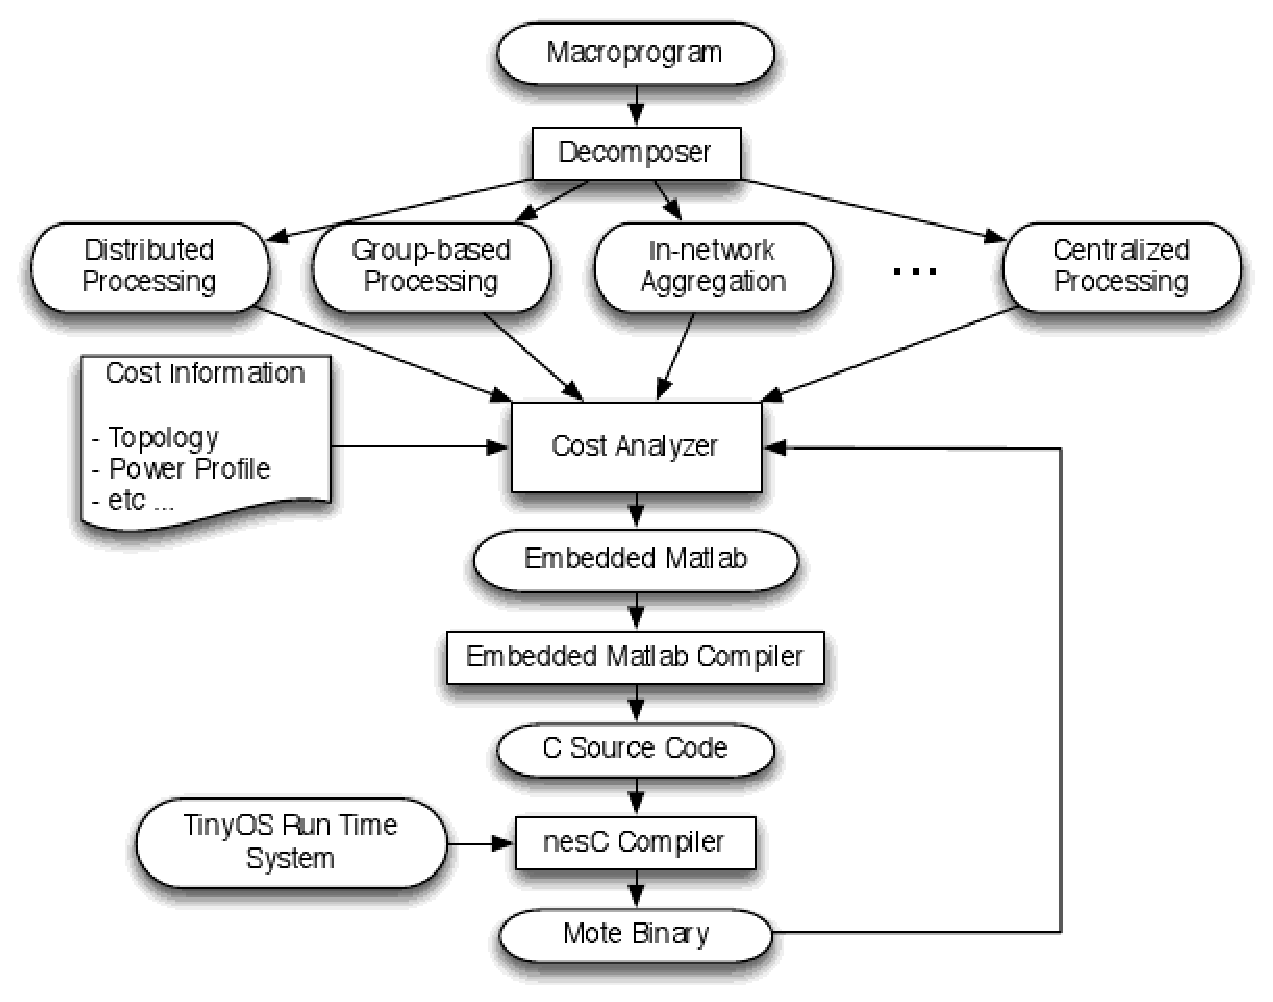
\includegraphics[width=0.8\columnwidth]{fig/System.eps}
  \caption[MacroLab system architecture]{MacroLab consists of a decomposer, a
  cost analyzer, and a run-time system. In our implementation, we generate all
  possible decompositions of a macroprogram and then analyze and compare them
  based on the cost profile of a target deployment.}
  \label{fig:System}
\end{figure}

\begin{figure}
  \centering
  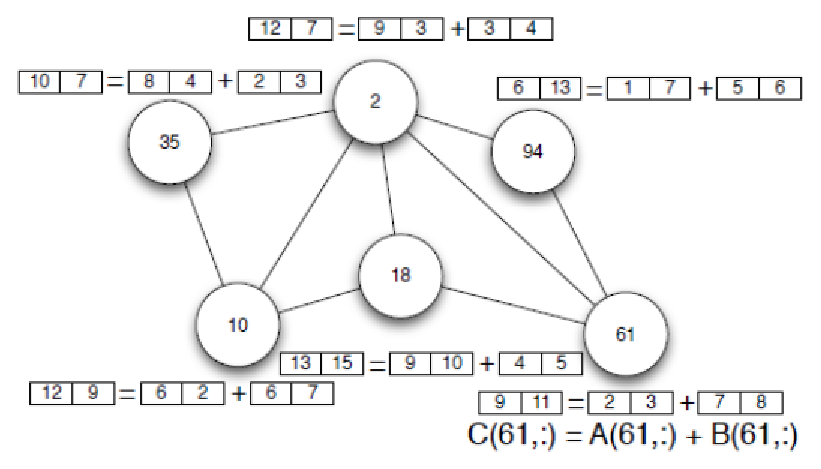
\includegraphics[width=0.8\columnwidth]{fig/DistributedArray.eps}
  \caption[Distributed Macrovector]{Distributed Macrovector: Nodes can read and write their own values in
  the vector.}
  \label{fig:distributedVector}
\end{figure}

\begin{figure}
  \centering
  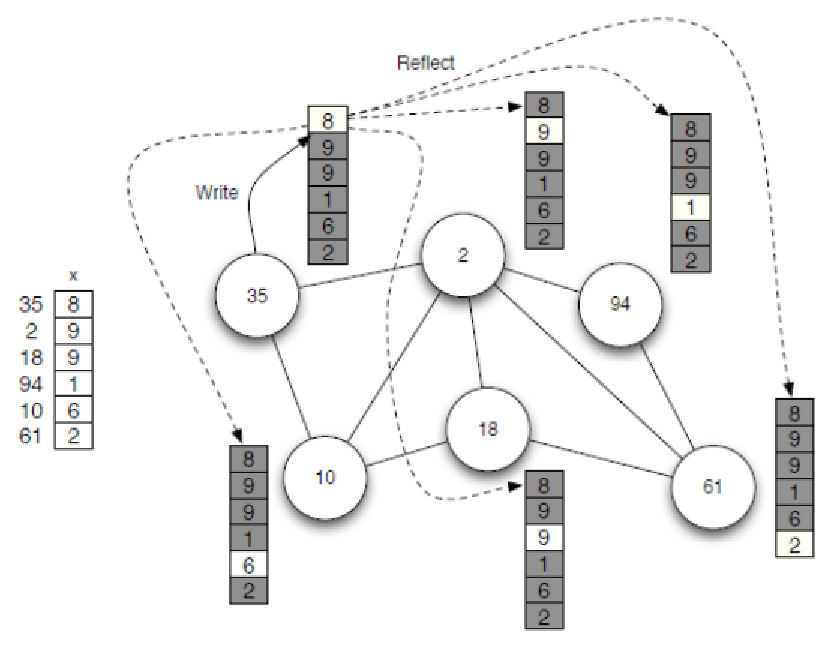
\includegraphics[width=0.8\columnwidth]{fig/ReflectedArray.eps}
  \caption[Reflected Macrovector]{Reflected Macrovector: Nodes can read all values in the vector, but can only write to their own value.}
  \label{fig:reflectedVector}
\end{figure}

\begin{table}
  \centering
   \begin{tabular}{| l |}
     \hline
     \multicolumn{1}{|c|}{Operation} \\
     \hline
     getID() \\
     \textit{returns the node's ID}\\
     \hline
     getProperty('property') \\
     \textit{returns a generic property of a node} \\
     \hline
     getNodes('group') \\
     \textit{returns the current membership in a global group}\\
     \hline
     getTime() \\
     \textit{returns the current global time} \\
     \hline
     getNeighbors() \\
     \textit{returns the current radio neighbors of a node}\\
     \hline
     remoteFeval(nodeIDs,funcName,\{P1,P2,...,Pn\}) \\
     \textit{remote function invocation}\\
     \hline
   \end{tabular}
   \caption[Functions supported by the Run-Time System]{The RTS must provide an interface for
   neighbor discovery, time sync, and remote function calls.}
   \label{table:lib}
\end{table}

\begin{table}
\begin{tabular}{|l|l|l|}
\noalign{\hrule} 
 & & \multicolumn{1}{c|}{$\mathbf{lhs = M(a_1,\ldots,a_n) \ \% \ Synchronous\ Read }$ } \\
\noalign{\hrule}
\multirow{2}{*}{\begin{sideways}Cnt. or Ref.\end{sideways}} & R& %
\tt\begin{tabular}{l} %
owner\_id = RTS.owner(cur\_pc(), M); \\
RTS.notify(cur\_pc(), owner\_id); \\
\end{tabular} \\ \cline{2-3}
 & L & %
% Centralized, local (i.e. we have control)
\tt\begin{tabular}{l} %
node\_ids = source\_nodes(a1); \\
RTS.wait(cur\_pc(), node\_ids); \\
lhs = local( M(a1,...,an) ); \\
\end{tabular} \\ \noalign{\hrule}
\multirow{2}{*}{\begin{sideways}Distributed\end{sideways}} & R & %
\tt\begin{tabular}{l} %
if (a1 contains node\_id()) then \\
~~owner\_id = RTS.owner(cur\_pc(), M); \\
~~RTS.send(owner\_id, \\
~~~~local(M(node\_id(), a2,...,an) )) \\
~~RTS.notify(cur\_pc(), owner\_id); \\
fi; \\
\end{tabular} \\ \cline{2-3}
 & L &  %
\tt\begin{tabular}{l}%
node\_ids = source\_nodes(a1); \\
RTS.wait(cur\_pc(), node\_ids); \\
lhs = local( M(a1,...,an) ); 
\end{tabular}   \\
\noalign{\hrule}
\end{tabular}
\caption[Pseudocode for mote-level microcode translation of synchronous read] {For each data representation, the row
marked L (for \emph{local}) denotes the code for the mote that will
perform the operation (i.e., the locus of synchronization); R (for
\emph{remote}) marks the code for all other nodes. {\tt M} is a
macrovector; {\tt lhs} and {\tt rhs} are normal vectors. The
mote-local representation of {\tt x} is given by {\tt local(x)}. The
{\tt owner(PC,M)} function gives the ID of the node requesting
the read or write operations on macrovector {\tt M} at
location {\tt PC} in the macroprogram.}
\label{table:synchronousRead}
\end{table}

\begin{table}
\begin{tabular}{|l|l|l|}
\noalign{\hrule} 
 & & \multicolumn{1}{c|}{$\mathbf{M(a_1,\ldots,a_n) = rhs \ \% \ Synchronous\ Write}$ } \\
\noalign{\hrule}
\multirow{2}{*}{\begin{sideways}Centralized\end{sideways}} & R& %
\tt\begin{tabular}{l} %
if (a1 contains node\_id()) then\\
~~owner\_id = RTS.owner(cur\_pc(), M); \\
~~RTS.wait(cur\_pc(), owner\_id); \\
fi; \\
\end{tabular} \\ \cline{2-3}
 & L & %
\tt\begin{tabular}{l} %
node\_ids = source\_nodes(a1); \\
local( M(a1,...,an) ) = rhs; \\
RTS.notify(cur\_pc(), node\_ids); \\
\end{tabular} \\ \noalign{\hrule}
\multirow{2}{*}{\begin{sideways}Reflected\end{sideways}} & R & %
\tt\begin{tabular}{l} %
if (a1 contains node\_id()) then \\
~~owner\_id = owner(cur\_pc(), M); \\
~~RTS.receive(owner\_id, \\
~~~~local( M(a1,...,an) )); \\
~~RTS.wait(cur\_pc(), owner\_id); \\
fi; \\
\end{tabular} \\ \cline{2-3}
 & L & %
\tt\begin{tabular}{l} %
node\_ids = source\_nodes(a1); \\
local( M(a1,...,an) ) = rhs; \\
foreach (node\_id in node\_ids) do \\
~~RTS.send(node\_id, \\
~~~~~~~~~~~local( M(a1,...,an) )); \\
done; \\
RTS.notify(cur\_pc(), node\_ids); \\
\end{tabular} \\ \noalign{\hrule}
\multirow{2}{*}{\begin{sideways}Distributed\end{sideways}} & R & %
\tt\begin{tabular}{l} %
if (a1 contains node\_id()) then \\
~~owner\_id = RTS.owner(cur\_pc(), M); \\
~~RTS.receive(owner\_id, \\
~~~~local(M(node\_id(), a2,...,an))); \\
~~RTS.wait(cur\_pc(), owner\_id); \\
fi; \\
\end{tabular} \\ \cline{2-3}
 & L &  %
\tt\begin{tabular}{l}%
node\_ids = source\_nodes(a1); \\
local( M(a1,...,an) ) = rhs; \\
foreach (node\_id in node\_ids) do \\
~~RTS.send(node\_id,\\
~~~~~~~~~~~local( M(a1,...,an) )); \\
done; \\
RTS.notify(cur\_pc(), node\_ids); \\
\end{tabular}   \\
\noalign{\hrule}
\end{tabular}
\caption[Pseudocode for mote-level microcode translation of synchronous write] {For each data representation, the row
marked L (for \emph{local}) denotes the code for the mote that will
perform the operation (i.e., the locus of synchronization); R (for
\emph{remote}) marks the code for all other nodes. {\tt M} is a
macrovector; {\tt lhs} and {\tt rhs} are normal vectors. The
mote-local representation of {\tt x} is given by {\tt local(x)}. The
{\tt owner(PC,M)} function gives the ID of the node requesting
the read or write operations on macrovector {\tt M} at
location {\tt PC} in the macroprogram.}
\label{table:synchronousWrite}
\end{table}

\begin{figure}
  \begin{nesc}
module LightSensorP {
  provides interface LightSensor;
  uses interface Read<uint16_t> as Read;
}
implementation
{
  command void LightSensor.sense() {
    call Read.read();
  }
  event void Read.readDone(error_t err,
   uint16_t val) {
    if(err == SUCCESS) {
      #CALLBACK(val);
    }
  }
}
  \end{nesc}
  \caption[A split-phase hardware driver for reading from the light sensor]{The
  {\tt LightSensor.sense} function is called by the microcode through the RTS.
  The decomposer must automatically replace {\tt\#CALLBACK} with an appropriate
  function to continue microprogram execution.}
  \label{code:hardwareDriver}
\end{figure}

\begin{figure}
  \begin{macrolab}
RTS = RunTimeSystem();
lSensors = SensorVector('lightSensor','uint16');
lightValues = Macrovector('uint16');
every(1000)
  lightValues =  sense(lSensors);
  BASE_DISPLAY(lightValues);
end
  \end{macrolab}
  \caption[A data collection application (Surge) in MacroLab]{Surge reads sensor
  values and displays them at the base station.  {\tt BASE\_DISPLAY} is
  implemented within the RTS and sends a message to a base station for display.}
  \label{code:Surge}
\end{figure}

\begin{figure}  
  \begin{macrolab}
motes = RTS.getMotes('type', 'tmote')
magSensors = SensorVector(motes, 'magnetometer');
magVals = Macrovector(motes);
neighborMag = neighborReflection(motes, magVals);
THRESH = uint8(500);
every(1000)
  magVals =  magSensors.sense();
  active = find(sum(neighborMag > THRESH, 2) > 3);
  maxNeighbor = max(neighborMag, 2);
  leaders = find(maxNeighbor(active) == magVal(active));
  CAMERAFOCUS(leaders);
end
  \end{macrolab}
  \caption[A tracking application (PEG) in MacroLab]{Every 1000\ms, nodes take a
  reading from their magnetometers and share the values with their neighbors.
  If more than three nodes in a neighborhood sense a magnetometer value about a
  threshold, a leader is elected from among them and a camera is focused on
  it. {\tt CAMERAFOCUS} is implemented within the RTS and sends a message to the
  camera, which is at the base station.}
  \label{code:PEG}
\end{figure}

\begin{figure*}[t]
  \begin{macrolab}
    RTS = RunTimeSystem();
    busstops = RTS.getNodes('stopnode'); 
    buses = RTS.getNodes('bus');
    estimates = Macrovector(busstops, length(buses) ,'uint16');
    arrivals = Macrovector(busstops, length(buses) ,'uint16'));
    travelTime = Macrovector(busstops, length(busstops), length(buses) ,'uint16'));
    busSensors = SensorVector('BusSensor',busstops,'uint16');
    routes = uint8({[1 2 3 4], [ 5 6 7 8]}); %Example routes

    while(1)
      [busID,r] =  sense(busSensors);
      busTime = RTS.getTime();
      travelTime(routes{r},routes{r},busID)[1,3] = busTime - arrivals(routes{r}, busID);
      arrivals(routes{r},busID)[1,2] = busTime;
      estimates(routes{r},busID) = travelTime(routes{r},routes{r},busID)[2,3] + busTime;
      BASE_DISPLAY(estimates(routes{r},:));
    end
  \end{macrolab}
  \caption[A bus tracking application in MacroLab]{MacroLab code for the bus
  tracking application.}
  \label{code:BusTracking}
\end{figure*}
